\documentclass[11pt, oneside]{article} 
\usepackage{mathptmx}
\usepackage{amsmath, amsthm, amssymb, calrsfs, wasysym, verbatim, bbm, color, graphics, geometry}
\usepackage{graphicx}
\usepackage{float}
\usepackage{longtable}
\usepackage{rotating}
\usepackage{adjustbox}
\usepackage{booktabs}
\usepackage{caption}
\usepackage[english]{babel}
\usepackage[utf8]{inputenc}
\usepackage[table]{xcolor}
\usepackage{multicol}
\usepackage{hyperref}
\usepackage{amsmath}

\geometry{tmargin=.75in, bmargin=.75in, lmargin=.75in, rmargin = .75in}  

\newcommand{\R}{\mathbb{R}}
\newcommand{\C}{\mathbb{C}}
\newcommand{\Z}{\mathbb{Z}}
\newcommand{\N}{\mathbb{N}}
\newcommand{\Q}{\mathbb{Q}}
\newcommand{\Cdot}{\boldsymbol{\cdot}}

\newtheorem{thm}{Theorem}
\newtheorem{defn}{Definition}
\newtheorem{conv}{Convention}
\newtheorem{rem}{Remark}
\newtheorem{lem}{Lemma}
\newtheorem{cor}{Corollary}

\font\arial=cmr12 at 40pt
\title{{\arial AN2DL Second Homework}}
\font\calibri=cmr12 at 20pt
\author{{\calibri Mauro Famà,   Sofia Martellozzo,   Lorenzo Mondo\\ \\
        Group cANNoli}}
\date{Academic Year 2022-2023}

\begin{document}

\maketitle
\begin{center}
    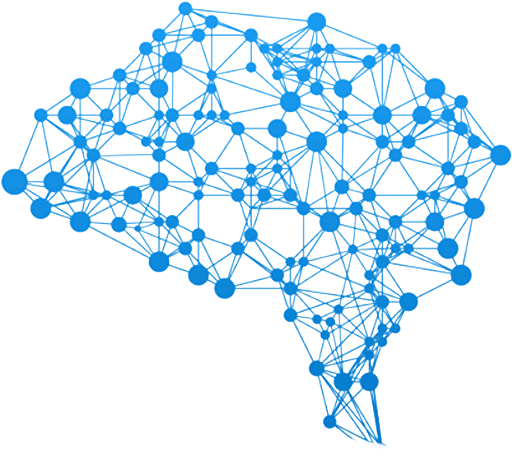
\includegraphics[scale=0.43]{images/title.png}
\end{center}
\newpage
\vspace{.25in}

%---------------------------------------%

\section{Introduction}

%---------------------------------------%
\section{Techniques}
\subsection{Data Augmentation}



%---------------------------------------%
\section{Development Models}

%---------------------------------------%
\section{Final Model}

%---------------------------------------%
\section{Conclusions}

%---------------------------------------%
\section*{References}
[0] 
{[1]} 
{[2]}
\end{document}
